%% Template made by Antonius Torode

\documentclass[11pt]{article}

%%% These are some packages that are useful
\usepackage{amsmath,amssymb, amscd,amsbsy, amsthm, enumerate}
\usepackage[export]{adjustbox}
\usepackage{lastpage}
\usepackage[top=1in, bottom=1in, left=1in, right=1in]{geometry}
\usepackage[unicode]{hyperref}
\usepackage{tikz, pgfplots, xcolor, fancyhdr}
\usepackage{multicol}
\usepackage{lipsum}

%%% Page formatting
%\setlength{\headsep}{30pt}
\setlength{\textheight}{9in}
\newcommand{\tab}{\hspace{1cm}}
%\setlength{\parindent}{25pt}

\title{Magnetic Storage, and Underlying Principles Therin}
\author{Parker Brue}

%%% Header and Footer Info
\pagestyle{fancy}
\fancyhead[L]{{\large PHY 482 }}
\fancyhead[C]{\today}
\fancyhead[R]{Name: Parker Brue}
\fancyfoot[L]{MSU}
\fancyfoot[C]{}
\fancyfoot[R]{\thepage\ of \pageref{LastPage}}

%% Use these two lines to remove the header
%\fancyhf{} % sets both header and footer to nothing
%\renewcommand{\headrulewidth}{0pt}

% Used to define spacing and format of References
\let\OLDthebibliography\thebibliography
\renewcommand\thebibliography[1]{
	\OLDthebibliography{#1}
	\setlength{\parskip}{0pt}
	\setlength{\itemsep}{0pt plus 0.3ex}
}



%%% Document Starts now
\begin{document}

\maketitle
\begin{abstract}
Magnetic storage, an essential part of a technologically integrated life, serves as a showcase of the far reaching properties of electromagnetism. The storage component relies on the semi-permanent qualities of magnetic hysteresis to manipulate magnetic media. Reading and writing to magnetic media capitalizes on magnetic flux, by moving the magnetic media relative to a sensor head. The development of the giant magneto-resistive based sensor heads alongside improved magnetic media are the primary factors in minimizing space and maximizing sensitivity in magnetic storage, though we are rapidly approaching a hard theoretical limit.  The principles discussed above are presented in reasonable depth and connected to fundamental concepts in undergraduate physics.
\end{abstract}
\thispagestyle{fancy}

\begin{multicols}{2} %begin multiple columns
From holding music, photographs, and other important documents at home, to providing the basis of magnetic strip identification cards, the proliferation of magnetic storage is easily one of the biggest additions to a technologically integrated life. Magnetic storage exploits the properties of magnetization and electrodynamic interactions in systems to provide dense and rapid access of information, with the development of giant magneto-resistive based sensor heads only serving to improve these factors by several orders of magnitude.
\begin{center}
	\centering
	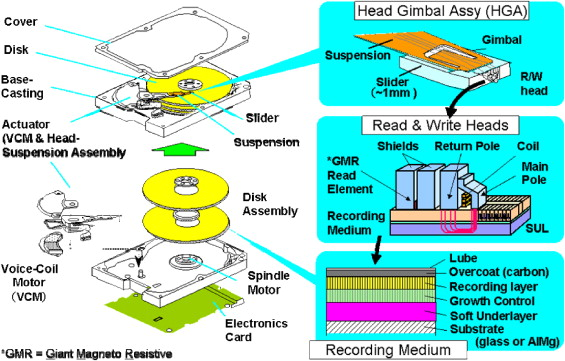
\includegraphics[width=0.48\textwidth]{HDD_makeup.png}
	{\footnotesize\textbf{Figure 1:} Breakdown of a HDD. The magnetic recording medium is found in the disks that spin in the HDD. The part where the EM phenomena takes place is an incredibly tiny Read and Write head\textsubscript{\cite{label6}}.}
\end{center} 
The most prominent usage of magnetic storage is that of a hard disk drive (HDD). It serves as an all-in-one package for the two most important aspects of magnetic storage; the storage in the medium itself, and the reading of and writing to the medium. Before delving into how data is interpreted, it is logical to first understand the mechanisms of storage.

On the surface level, the storage component of magnetic storage is fairly straightforward. Ferromagnetic material, once induced with a magnetic field, will keep alignment with that magnetic field until sufficient heat or magnetization is provided to overcome the field strength. If an oppositely aligned magnetic field is strong enough, it breaks the alignment of the ferromagnetic material and establishes a field anti-parallel to the first one. Unless introduced to an intense degaussing magnetic field that breaks down magnetization, the ferromagnetic material will be stuck in either an anti-parallel or parallel alignment. This phenomenon of a semi-permanently aligned magnetic field is known as magnetic hysteresis. This forms the basis of magnetic storage, as permanently established localized differences in magnetic field orientation can be used to establish a readable pattern of data\textsubscript{\cite{label1}}.

\begin{center}
	\centering
	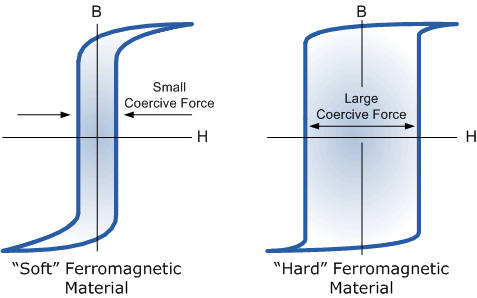
\includegraphics[width=0.48\textwidth]{mag_hysterisis.png}
	{\footnotesize\textbf{Figure 2:} Different ferromagnetic materials exhibit different coercivities, or the resistance a magnetic material has to changes in magnetization, this has a very wide application in magnetic storage, in both storage and sensor methods.\textsubscript{\cite{label7}}}
\end{center} 

It conceptually helps to break down the ferromagnetic medium into discrete chunks, or bits, that are a consequence of linear storage density and recorded wavelength. Linear storage density (k) is a product of wavelength ($\lambda$), medium speed (U), and recording frequency (f):
\begin{align*}
	\lambda= \dfrac{U}{f} = \dfrac{2}{k}
\end{align*}
This means the minimum recordable wavelength is dependent on how fast the medium is traveling and the recording frequency, so logically it follows that for higher linear density, it would benefit to run a drive at slow speed and record at a very high frequency. This is a trade-off for data access speeds, however\textsubscript{\cite{label1}}. Magnetic Tape drives have massive storage density in relative to HDDs, but a HDD operating at 7200 RPM is many times faster in random data access, a boon for the typical user. 

Once a recorded wavelength has been established, the discrete bit length is equivalent to half of the wavelength. A magnetic material on the bit is arranged in either a parallel or anti-parallel fashion. The interesting part is how these recorded bits are interpreted into binary code, a common method of interpretation is non-return to zero inverted (NRZI). Instead of what one may intuitively think how magnetic bits are translated, NRZI doesn't interpret 1 or 0 as parallel or anti-parallel. NRZI instead focuses on change of magnetization to create a waveform code, this is a more efficient process\textsubscript{\cite{label1}}. 

\begin{center}
	\centering
	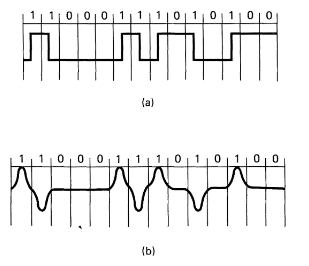
\includegraphics[width=0.48\textwidth]{Waveform_code.png}
	{\footnotesize\textbf{Figure 3:}  A) NRZI code and B) waveform of the current. 1 indicates a change in the magnetization recorded and 0 indicates no change. This leads to data reading functioning as a Toggle Flip-Flop that is, the NRZI code will stay on (1) until the opposite value is returned. Writing is done when the head current is powered strongly enough to invert the magnetic field of the bit\textsubscript{\cite{label1}}}.
\end{center} 

As figure 3 demonstrates, code that can be created in magnetic material. The process behind actually reading the code and changing the physical bits behind the code relies on the sensor head in figure 1. Reading and writing capitalize on the consequences of magnetic flux due to relative movement of or in a magnetic field. For a HDD in reading mode, parallel bits in the rotating medium induce looping current in the head in a direction dependent on the orientation of the bit. This current is then amplified and interpreted in a code such as NRZI. In writing mode, a current is induced in the head that creates fringe magnetic fields powerful enough to overwrite bits of the medium, utilizing magnetic hysteresis\textsubscript{\cite{label1}}.

Sensor heads rely on the quantum phenomena of giant magneto-resistance (GMR). GMR is crucial to sensing external magnetic fields at low field strengths and at small sizes minimally disrupting the field and medium containing the field. It was discovered by Grunberg and Fert through studying the interactions of layered sheets of Fe/Cr/Fe. It was found that anti-parallel magnetic alignment of the ferromagnetic layers results in a higher resistivity\textsubscript{\cite{label5}}. Experimental research is ongoing to find the optimal layer composition and layout, but the most useful structure is the subgroup of spin-valve sensors, which serve as the basis for Read/Write sensor heads in magnetic storage devices\textsubscript{\cite{label4}}.

In the Fuchs-Sondheimer model, GMR is evaluated by assuming that it's based upon spin-dependent scattering mechanisms, as well as the relative length of the mean free paths in relation to the thickness of various layers. The FS model is a highly simplified model of electron transport in thin metal films, only requiring the two aforementioned parameters in order to function. This means that while it works nicely in theory, it’s a lot harder to expand upon experimentally due to the myriad of interactive factors in a real metal film. Camley and Barnas take it upon themselves to expand upon the FS model to make it experimentally viable. They include spin-dependent coefficients for specular reflection, transmission, and diffuse scattering, by making the assumptions that the metals involved are equivalent simple metals, and that there is no angular dependence on scattering.The basis of computing the conductivity begins through application of the Boltzmann equation
\begin{align*}
\dfrac{dg}{dz}+ \dfrac{g}{\tau v_z} = \dfrac{eE}{m v_z} \dfrac{df_0}{dv_x}
\end{align*}
$f_0$ is the equilibrium distribution function, which accounts for the number of particles per unit volume, this is important for discussing conductivity in terms of scattering probabilities, as the particle density will influence scattering probability. $v_z$ is the velocity of the particle in the z direction.  The term g is the correction in the distribution function from an external E field in the x direction, this accounts for the scattering probabilities from particle and film orientation as a particle travels through a multilayer system. It should be noted that terms which involve magnetic field effects are discarded due to their irrelevant size in regard to the calculations done\textsubscript{\cite{label2}}. The Boltzmann equation is used because it offers a statistical look into charge transport, it portrays the probability of the electron to pass through various layers without getting deflected. In other words, the effective conductive ability of the system.

The value for g takes into account many contributions from spin up and spin down electrons moving in the positive and negative direction in the various layers, where we end up with about 8 different g contributions for the total correction. Once g is found, the current density, similar to  the simple cases in electromagnetism, can be evaluated:
\begin{align*}
J(z) = \int v_x g(v_z,z)d^3 v  
\end{align*}
Which can then be used to find the effective resistivity. The theory predicts that resistivity of magnetic layered systems depends on the diffusive scattering parameter, 
\begin{align*}
1-T \uparrow= D \uparrow
\end{align*}
\begin{align*}
N = D \uparrow D \downarrow 
\end{align*}
$D\uparrow$ is a measurement of interface roughness, and N is the asymmetry in up down scattering. An increase in $D\uparrow$ or N should also increase magnetoresistance\textsubscript{\cite{label2}}. This means that is a rougher surface should result in less conductivity. Examining conductivity from a statistical perspective, this makes sense, a rougher surface means that the electron is more likely to be repelled. 

Camley and Barnas measured the resistance change as a function of applied field, the angle used in the calculation of the magnetization differences was found through minimizing the sum of exchange, anisotropy, and Zeeman energies. The relative angle between the reference and free layer will determine the change in resistivity, and consequently, magnetization. As demonstrated by Camley and Barnas, the theoretical model is reasonably accurate in comparison to experimental results, but the differences can be accounted for the lack of incorporation of magnetoresistive anisotropy in the theoretical calculations. 

\begin{center}
	\centering
	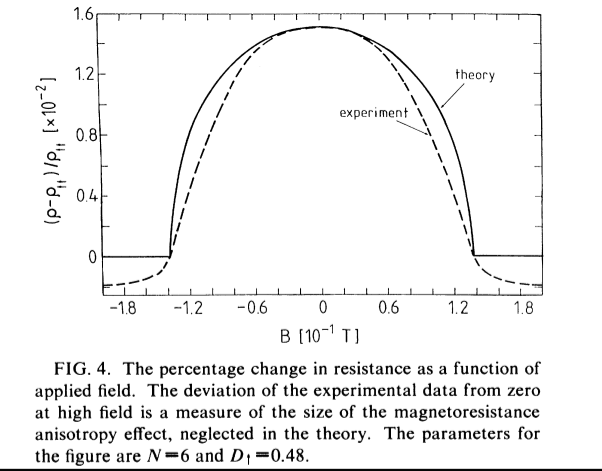
\includegraphics[width=0.48\textwidth]{exp_vs_theory.png}
	{\footnotesize\textbf \textsubscript{\cite{label2}}}
\end{center} 


The subgroup of GMR sensors, spin-valve sensors, at their most basic, comprise of a fixed magnetic layer, a nonmagnetic spacer, and a magnetic layer that can change its orientation\textsubscript{ \cite{label3}}. Measurements on magnetic fields are done through comparison of the magnetization vector of the free layer to the reference layer. GMR resistance values change based on the relative position of the free layer. So in practice, bits in the same alignment as the reference layer pass through a lower resistance, and bits in the opposite alignment will pass a higher resistance, usually around 10 percent of a change in total resistance, resulting in a basic sensitivity of 20 mV. The continuing experimental challenge is to make these sensors smaller even more sensitive to account for increased storage density\textsubscript{ \cite{label5}}.

\begin{center}
	\centering
	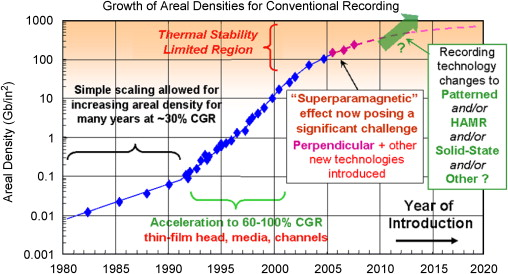
\includegraphics[width=0.48\textwidth]{region_of_stability.png}
	{\footnotesize\textbf{Figure 5:} The theoretical model of recording density growth begins to slow down as the superparamagnetic limit is approached, close to 1 Terabit/sq. in.. Higher densities simply result in thermally unstable materials as well as unusable signal-to-noise ratios. The huge jump in the 1990’s and mid 2000’s is due to the development and application of GMR sensors.\textsubscript{\cite{label6}}} 
\end{center} 

It is clear to see that magnetic storage is a powerful exploitation of electromagnetic systems, and while under close inspection falls into great depths of involvement, still relies on fundamental phenomena like magnetic hysteresis and the flux-current relation. Giant magneto-resistive sensor heads function as the capstone of pure HDD magnetic storage technology though deliverance to the theoretical limit. While HDDs may be reaching the peak of their theoretical development, they aren't going to be easily overtaken by newer solid state technology. The development of hybrid drives in recent years brings to the table a best of both worlds scenario, ensuring the relevancy of HDD magnetic storage technology for many years to come.


\begin{thebibliography}{9}
	{\footnotesize
	\bibitem{label1} Bhushan, Springer-Verlag, Tribology and Mechanics of Magnetic Storage Devices, Wiley, 1990, Section 1.3 
	\bibitem{label2} Camley, R. E., Theory of Giant Magnetoresistance Effects in Magnetic Layered Structures with Antiferromagnetic Coupling, Physical Review Letters, 08/1989, Volume: 63, Issue: 6, Pages: 664-667
	\bibitem{label3} Dieny, B, Giant Magnetoresistance in Spin-Valve Multilayers, Journal of Magnetism and Magnetic Materials, 09/1994, Volume: 136, Issue: 3, Pages: 335-359
	\bibitem{label4} Kools, J.C.S, Exchange-Biased Spin-Valves for Magnetic Storage, IEEE Transactions on Magnetics, 07/1996 Volume: 32 Issue: 4 Page: 3165
	\bibitem{label5}Weiss, et. al. Advanced Giant Magnetoresistance Technology for Measurement Applications, Measurement Science and Technology, July 2013.  
	\bibitem{label6} Wood, Roger, Future Hard Disk Drive Systems, Journal of Magnetism and Magnetic Materials, 03/2009, Volume: 321, Issue: 6, Pages: 555-561
	\bibitem{label7} Electronics Tutorial Team, "Magnetic Hysteresis Loop including the B-H Curve." Basic Electronics Tutorials. 05 Aug. 2016. Web. 01 Mar. 2017.
	
	}
\end{thebibliography}

\end{multicols}%end multiple columns

%%%%%%%%%%%%%%%%%%%%%%%%%%%%%%%%%%%%%%%%%%%%%%%%%%%%%%%%%%%%%%%%%%%%%%%%%%%%%%%%%%%%%%%%%%%
\end{document}





















